\chapter{Categorization API}
As mentioned before main purpose of this thesis is POI classification. Unfortunately main topic is difficult to isolate because it involves custom input data. In previous chapter preparation and implementation of custom input data was described. This chapter will cover the topic of categorization data which are already delivered to the system.

\section{POI Categories}

\subsection{Overview}
To effectively categorize POI there has to be defined appropriate category hierarchy. There are a lot of multiple standards which are widely used in many different solutions and technologies. Unfortunately there is no world-wide standard defined for POI categories. More frequent observation can be done when looking at companies like: \textbf{Garmin, TomTom, Waze} that those entities try to introduce their own solutions. Garmin offers its own \textit{POILoader} which allows for own category definition \cite{9}. On the other hand TomTom offers 500 different POI categories by default \cite{10} but if user is eager to add custom POIs additional steps need to be done. User must prepare his own files with extension \textbf{\textit{.ov2}} and deploy it on GPS device. What is more deployment process depend on device model. Waze also defines it's own POI category standard \cite{14} There is an endeavour done by \textbf{W3C} organization about standarizing POI Data Model unfortundately according do W3C wiki it is still in beta version and categories definied is supposed to be defined in future \cite{12}. Only XML standard was defined (which supposed to be used as world-wide standart for POI data transfer) \cite{13}
\begin{figure}
	\centering
	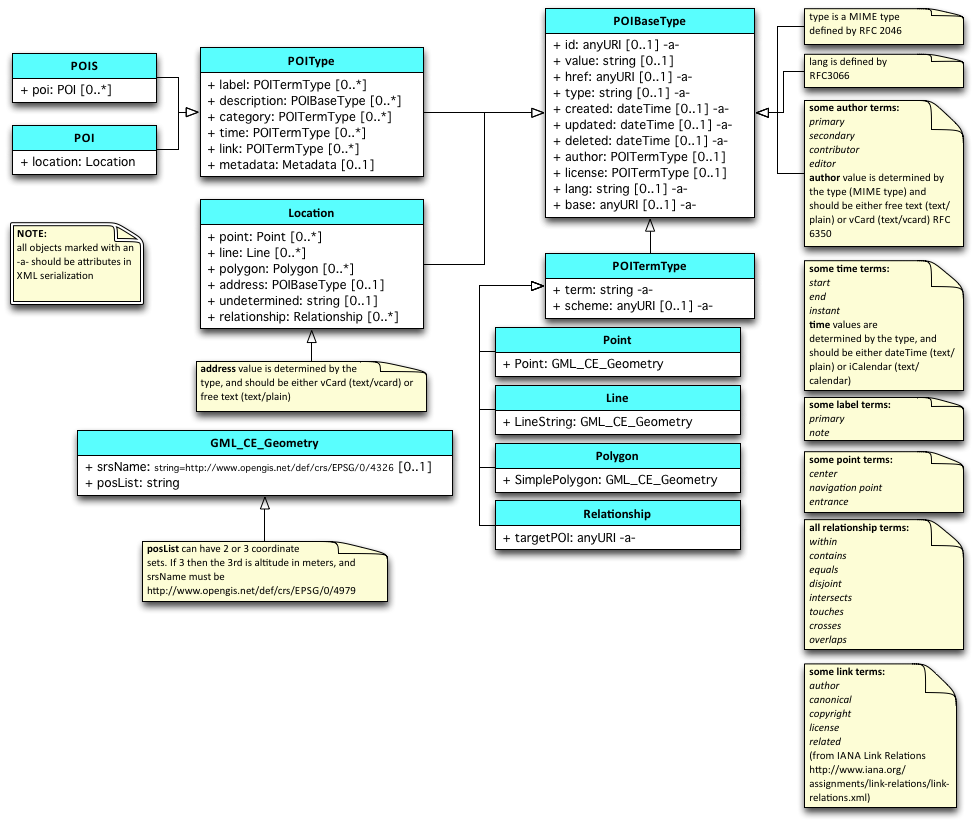
\includegraphics[scale=0.5]{W3c_poi_model.png}
	\caption{W3C UML Diagram POI Data Model}
	\label{fig:@=w3cDataModel}
\end{figure}
There is an apprehensible delamination in field of POI categories. It is difficult to find a standard which could be useful and well known for every data source. Fortunately there are standards defined by governments which describe categories in very detailed way and have endorsement by substantive position as countries governments possess. 
\subsection{NAICS}
\textit{\textbf{The North American Industry Classification System (NAICS)}} widely used in countries of North America. Developed by three organizations:  U.S. Economic Classification Policy Committee (ECPC), Statistics Canada, Mexico's Instituto Nacional de Estadistica y Geografia. It is mainly used by Federal agencies to collect data about bussiness entites for statistic purposes. It is successor of \textit{\textbf{Standard Industrial Classification (SIC)}}. NAICS classification is basing on codes which correspond to category description. Code can at most consist of six digits (the more digits included in code the more detailed category description is). Latest NAICS revision was issued in 2012. \cite{15} \cite{16}
\subsection{NACE}
\textit{\textbf{Statistical Classification of Economic Activities in the European Community (in French: Nomenclature statistique des activités économiques dans la Communauté européenne) - NACE}} system widely used in European Union. Similarly to NACE it is using combination of codes and category description. Code consists of letter and digits and creates special hierarchy of: sections, divisions, groups and classes. Section is marked by letter, division by two digits, groups and classes by one digit consecutively. Latest NACE revision (Rev.2) was issued in 2008 as a result of constantly developing and  newly appearing organizations especially in telecommunication business.\cite{17} \cite{18} Because java application which is purpose of this thesis was developed in Poland NACE categorization standard was chosen to apply in it. Obviously information included in NACE are definitely too much detailed to be applied for POI categorization system so only sections were taken into consideration. 

\section{Java library as categorization API}
\todo{cel api - zrodla danych, rezultat, metody processingu API = connection, classification, utilsy, czemu taki a nie inny podzial na pakiety - opis unit testow}
Main purpose of Java categorization API is to deliver an interface which would allow for convenient, correct and efficient results. API should be independent of data type which will be delivered. API responsibility is to enable functionalities (as this thesis states - categorization). To assure independence of data sources powerful mechanism of java interfaces can be used - such approach introduce level of abstraction and allow java library for easy communication with data sources. Java has very useful feature of importing and using libraries - when whole code is compiled to bytecode classes and bundled into resultant \textbf{\textit{.jar}} file - it can be immediately used in another java project by another programmer. Moreover, resultant java library project can be compiled with dependencies so programmer who will use library later will not have to bother about classes which were used during library development are were not part of Java API \cite{19}.   

\subsection{Packages organization}
API is divided into three packages: connection, classification and utils. Such packaging organization assures clear and concise presentation of API functionalites and utilities. Functional packages are divided into simillar hierachy to interfaces and packages responsible for particular data source handling. For purpose of this thesis these packages were named \textit{loadstone}. Obviously unit tests for corresponding executing classes are located into separate directory (according to maven directory structurce \cite{20}) but are included in the same package namespace.
\begin{figure}
 	\centering
 	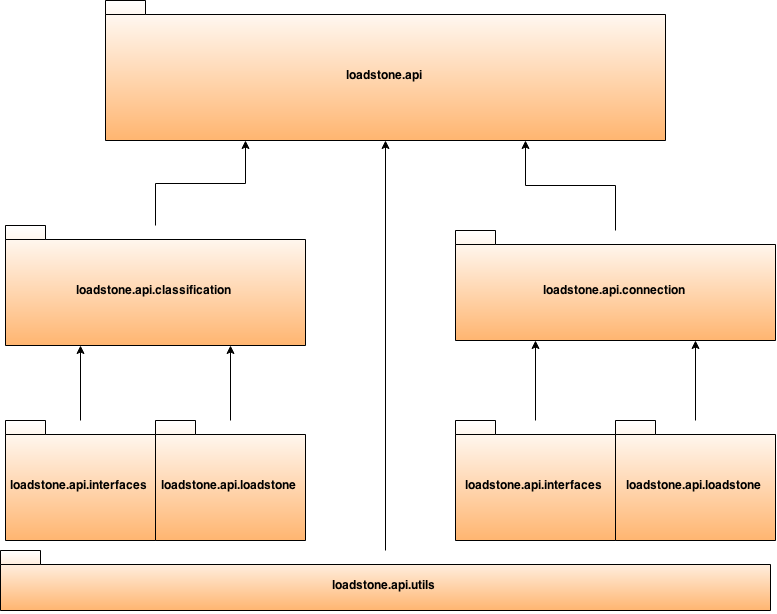
\includegraphics[scale=0.5]{packages_orgazniation.png}
 	\caption{Loadstone API packages organization}
 	\label{fig:@=packages_oragnization}
\end{figure}
\subsection{AbstractResourcePreprocessing Interface}
As mentioned before independence of input data is absolutely compulsory for API. To define preprocessing for each different kind data source  AbstractResourcePreprocessing interface was defined. Classes which will be strictly delegated to preprocess particular source of data by implementation of this interface will be able to communicate with API and pass already preprocessed data for further classification methods. \todo{jakis uml z interfejsem}
\subsection{LoadstonePreprocessing}
\todo{opis preprocessingu - klasy javowe oraz skrypt bashowy analyzeDB.sh} 

\subsection{Kolejne metody}
\todo{Inne metody processingu do zaimplementowania}